\documentclass[aspectratio=169]{beamer}

\usepackage[utf8]{inputenc}
\usepackage[spanish]{babel}
\usepackage{graphicx}
\usepackage{booktabs}
\usepackage{ragged2e}
\usepackage{minted}
\usepackage{xcolor}
\usepackage{tikz}
\usepackage{algorithm}
\usepackage{algorithmic}
\usepackage{minted}
\usepackage{listings}
\usepackage{tikz}
\usetikzlibrary{arrows.meta,positioning,fit,shapes.symbols}
\usetikzlibrary{arrows,shapes}
\definecolor{LightGray}{gray}{0.975}
\definecolor{links}{HTML}{2A1B81}
\hypersetup{colorlinks,linkcolor=,urlcolor=blue}

\usefonttheme{serif} 

\title[ETL]{Database Administration}
\subtitle{Lecture 05: ETL -- \underline{E}xtraction, \underline{T}ranformation \& \underline{L}oad}
\author{Kimball, Caserta \& Roldán}
\date{\today}

\setbeamertemplate{navigation symbols}{}%remove navigation symbols

\defbeamertemplate*{footline}{shadow theme}
{%
  \leavevmode%
  \hbox{\begin{beamercolorbox}[wd=.5\paperwidth,ht=2.5ex,dp=1.125ex,leftskip=.3cm plus1fil,rightskip=.3cm]{author in head/foot}%
    \usebeamerfont{author in head/foot} Database Administration \hfill \insertshorttitle
  \end{beamercolorbox}%
  \begin{beamercolorbox}[wd=.5\paperwidth,ht=2.5ex,dp=1.125ex,leftskip=.3cm,rightskip=.3cm plus1fil]{title in head/foot}%
    \usebeamerfont{title in head/foot} \hfill \insertframenumber\,/\,\inserttotalframenumber%
  \end{beamercolorbox}}%
  \vskip0pt%
}

\AtBeginSection[]
{
     \begin{frame}<beamer>
     \frametitle{Plan}
     \tableofcontents[currentsection]
     \end{frame}
}

\newcommand{\toRight}[1]{
    \begin{FlushRight}
        {\tiny #1}
    \end{FlushRight}
} % Align to right

\begin{document}

\frame{\titlepage}

\begin{frame}{Database Administration: ETL -- \underline{E}xtraction, \underline{T}ranformation \& \underline{L}oad.}
    \centering
    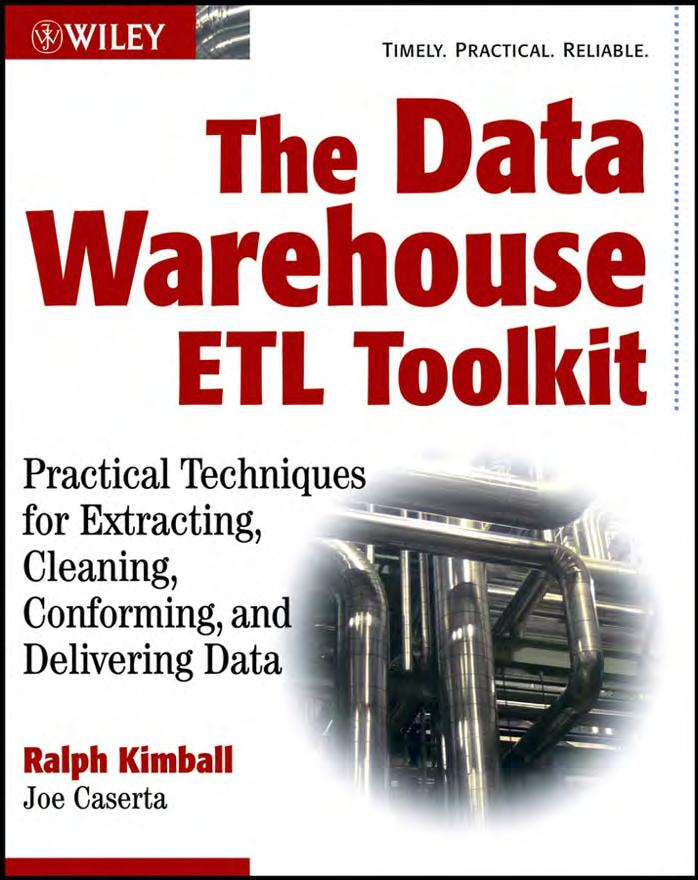
\includegraphics[width=0.3\textwidth]{figures/book_cover5}
    \hspace{5mm}
    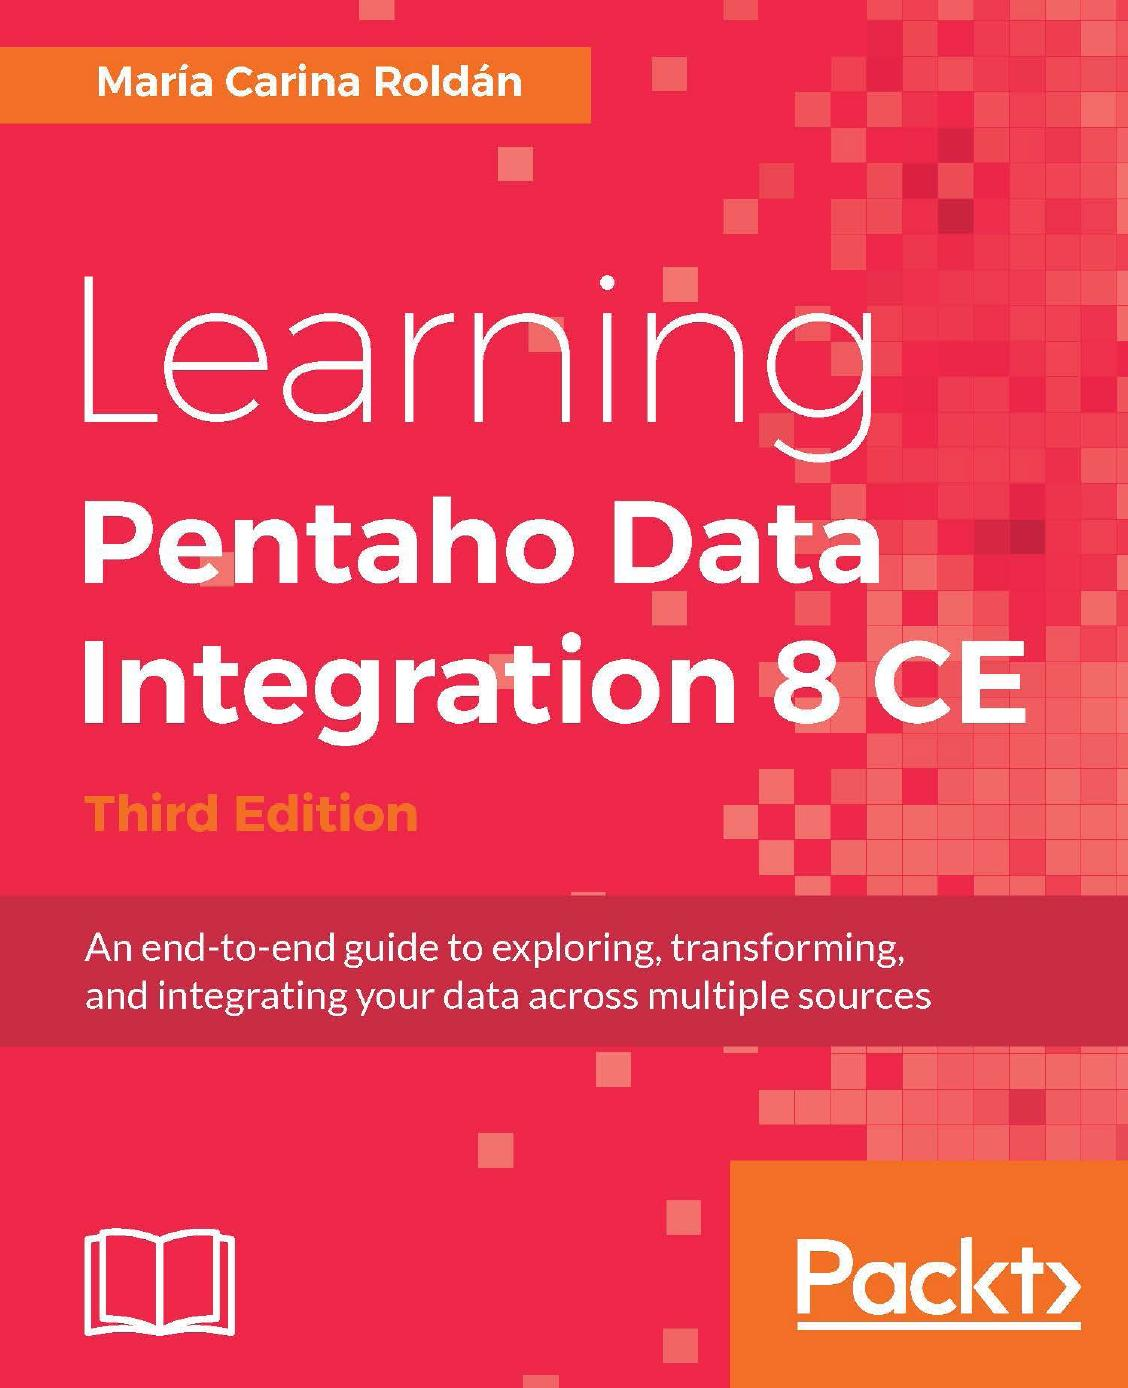
\includegraphics[width=0.3\textwidth]{figures/book_cover6} \\
    \vspace{1mm}
    {
        \scriptsize
        Content has been extracted from \textit{``The Data Warehouse ETL Toolkit''} by Kimball \& Caserta, 2004. Visit \href{https://www.kimballgroup.com/data-warehouse-business-intelligence-resources/books/data-warehouse-dw-etl-toolkit/}{kimballgroup.com}
        and
        \textit{``Learning Pentaho Data Integration 8 CE''} by Roldán, 2018. Visit \href{https://www.oreilly.com/library/view/learning-pentaho-data/9781788292436/a364bedc-72f6-4ccb-94a7-74c499bda3c4.xhtml}{oreilly.com}.
    }
\end{frame}

%%%%%%%%%%%%%%%%%%%%%%%%%%%%%%%%%%%%%%%%%%%%%%%%%%%%%%%%%%%%%%%%%%%%%%%%%%%%%

\begin{frame}{What is a Data Warehouse?}
\begin{itemize}
  \item \textbf{Purpose:} Publish organizational data assets to support decision-making.
  \item \textbf{Core traits:} Subject/process-oriented, integrated, time-variant, non-volatile.
  \item \textbf{Users:} Analysts, managers, apps (dashboards, reports, OLAP, data science).
  \item \textbf{Outcomes:} Trusted metrics, faster insight, single version of the truth.
\end{itemize}
\end{frame}

\begin{frame}{Main Components (Kitchen \& Dining Metaphor)}
    \textbf{Back Room (Kitchen)}
    \begin{itemize}
        \item Staging \& processing area (no end-user access)
        \item Raw sources $\rightarrow$ standardized, high-quality data
        \item Governance: lineage, quality checks, security, restart/recovery
    \end{itemize}
    \textbf{Front Room (Dining room)}
    \begin{itemize}
        \item Dimensional models / data marts (atomic + aggregates)
        \item Access by BI tools: SQL, reports, dashboards, OLAP, ML
        \item Performance tuning, semantic consistency (\emph{conformed} dims/facts)
    \end{itemize}
\end{frame}

\begin{frame}{DW Schema}
    \centering
    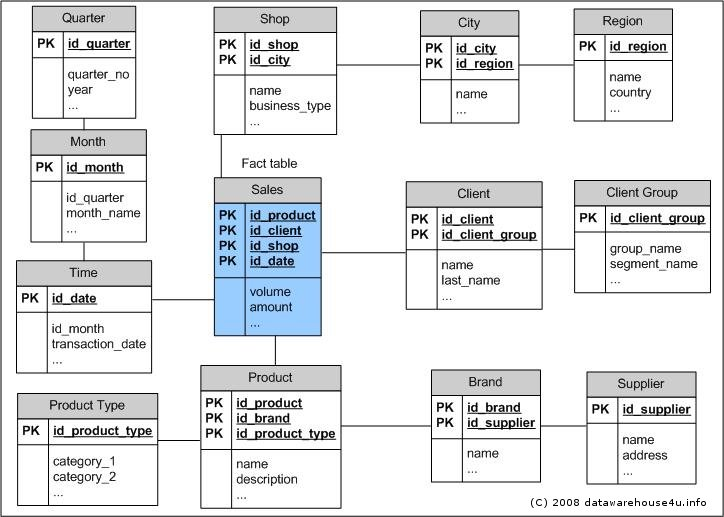
\includegraphics[width=0.7\textwidth]{figures/dw_schema}
\end{frame}

\begin{frame}{ETL Responsibilities}
    \begin{itemize}
        \item Add value: quality, standard units, surrogate keys, SCDs
        \item Preserve lineage \& auditability; archive staging
        \item Automate: scheduling, exceptions, recovery/restart
        \item Meet \textbf{latency} needs: batch or streaming (real-time)
    \end{itemize}
\end{frame}

\section{Main Requirements}

\begin{frame}{Why Requirements Matter}
    \begin{itemize}
        \item ETL design begins with surrounding the requirements.
        \item Requirements are non-negotiable constraints to adapt to.
        \item Early architectural decisions drive:
        \begin{itemize}
            \item Hardware \& software
            \item Coding practices
            \item Personnel \& operations
        \end{itemize}
        \item Clear mission: define back room, staging, operational data stores, presentation area.
    \end{itemize}
\end{frame}

\section{Categories of Requirements}

\begin{frame}{Business Needs}
    \begin{itemize}
        \item End users’ information requirements.
        \item Business needs drive the choice of data sources.
        \item Interviews and investigations often uncover:
        \begin{itemize}
            \item Hidden complexities or limitations
            \item Additional capabilities of data sources
        \end{itemize}
        \item Continuous dialogue between ETL team, architects, and end users.
    \end{itemize}
\end{frame}

\begin{frame}{Compliance \& Security}
    \begin{itemize}
        \item Sarbanes–Oxley and other regulations demand:
        \begin{itemize}
            \item Proof of accuracy, completeness, and lineage.
            \item Archived copies and documented algorithms.
        \end{itemize}
        \item Security:
        \begin{itemize}
            \item Role-based access control (via directory server).
            \item Separate ETL subnets, controlled backups, logs.
        \end{itemize}
    \end{itemize}
\end{frame}

\begin{frame}{Other Requirements}
    \begin{itemize}
        \item \textbf{Data Profiling:} assess quality, completeness, and usability.
        \item \textbf{Integration:} conforming dimensions \& facts.
        \item \textbf{Latency:} batch vs streaming delivery.
        \item \textbf{Archiving \& Lineage:} keep staged data + metadata.
        \item \textbf{End User Interfaces:} responsibility of ETL to simplify delivery.
        \item \textbf{Skills \& Legacy:} staff expertise and existing licenses impact design.
    \end{itemize}
\end{frame}

\section{Architectural Decisions}

\begin{frame}{ETL Tool vs. Hand Coding}
    \textbf{ETL Tool Advantages:}
    \begin{itemize}
        \item Faster development, metadata management.
        \item Built-in scheduling, connectors, lineage tracking.
        \item Good performance at scale.
    \end{itemize}
    \textbf{Hand-Coded Advantages:}
    \begin{itemize}
        \item Unlimited flexibility, OOP, unit testing.
        \item Full control over metadata.
        \item Avoid vendor lock-in.
    \end{itemize}
\end{frame}

\begin{frame}{Other Architectural Issues}
    \begin{itemize}
        \item Proven technology vs. untested tools.
        \item Batch vs. Streaming data flows.
        \item Task dependency: Horizontal vs. Vertical (latency vs consistency).
        \item Scheduler automation and monitoring.
        \item Exception handling, quality management, recovery.
        \item Metadata repositories and process-flow tracking.
    \end{itemize}
\end{frame}

\section{Back Room \& Front Room}

\begin{frame}{The Back \& Front Rooms}
    \centering
    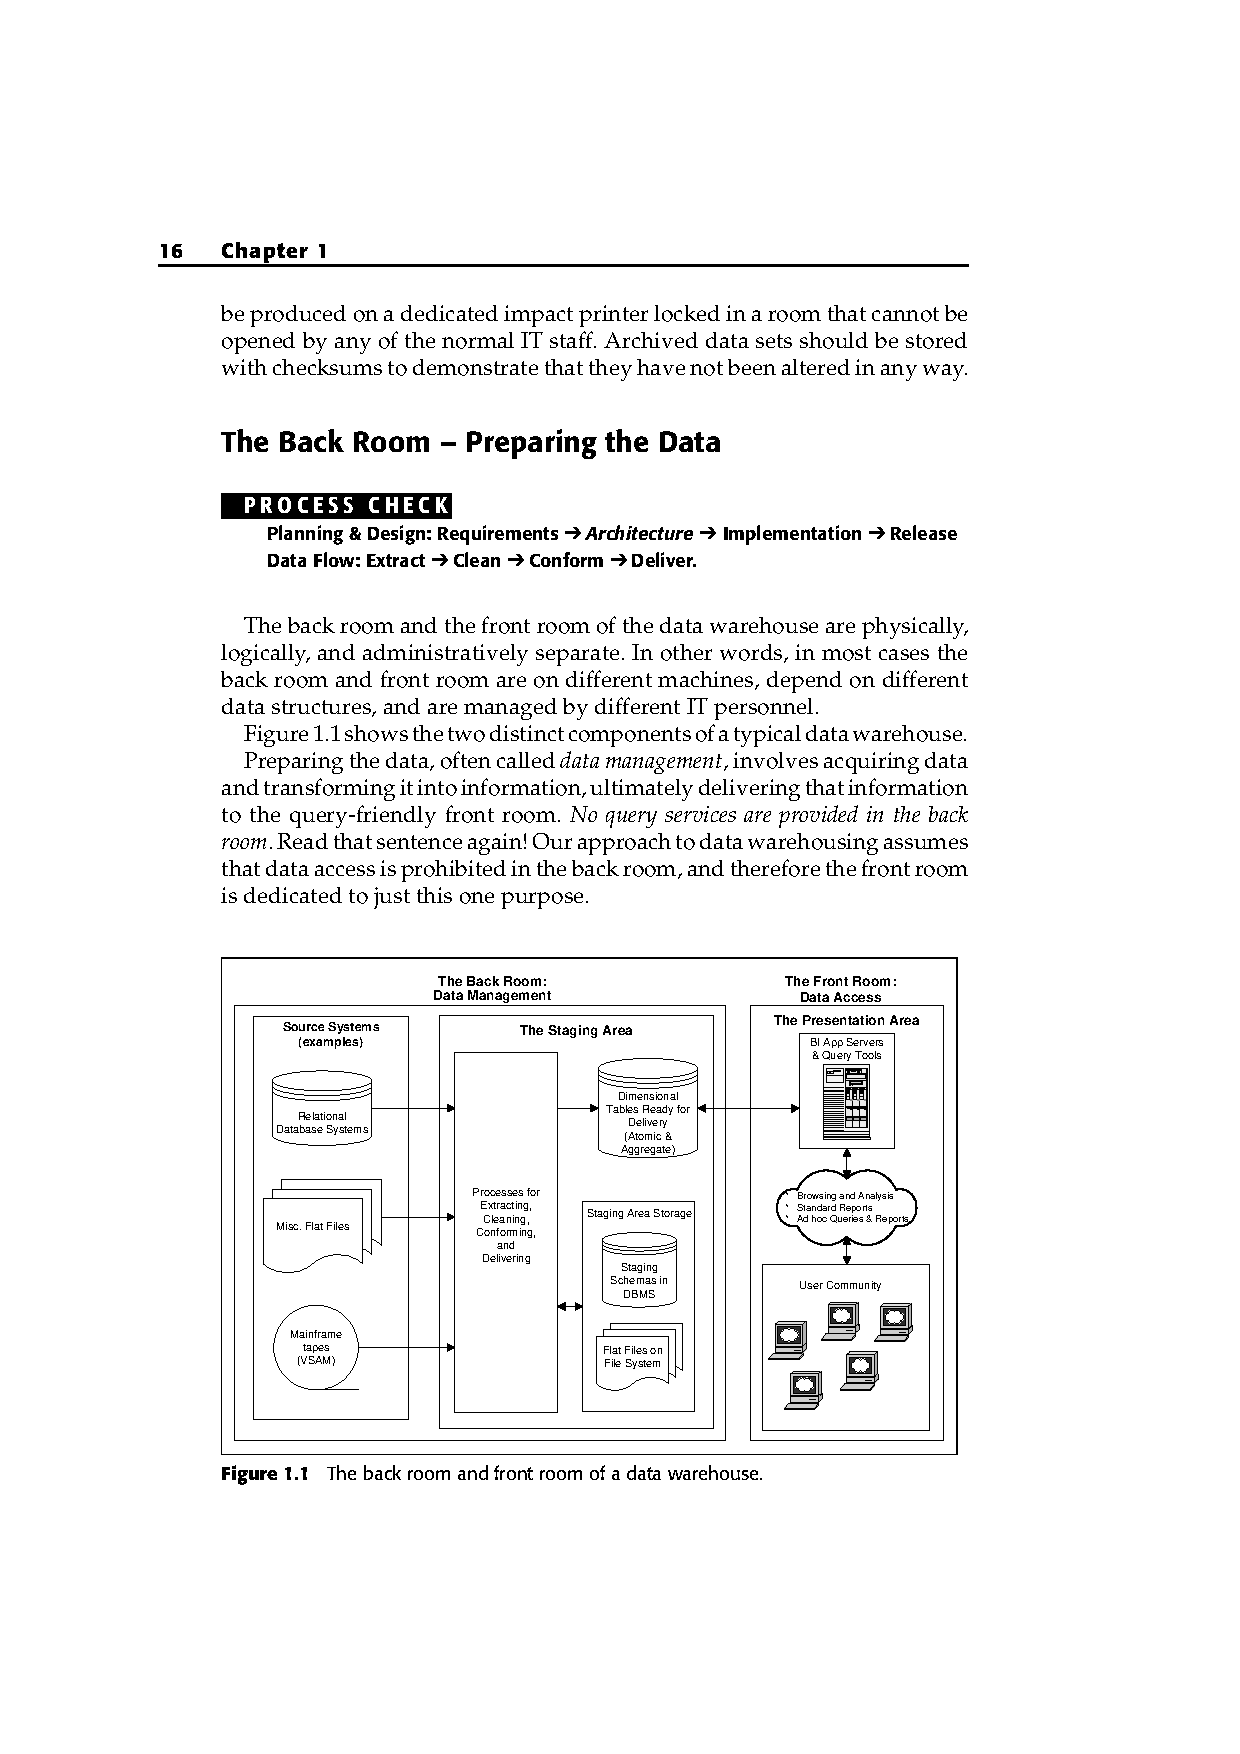
\includegraphics[width=0.8\textwidth, trim={3.5cm 4.55cm 3.5cm 16cm}, clip]{figures/rooms}
\end{frame}

\begin{frame}{The Back Room – Data Management}
    \begin{itemize}
        \item Kitchen metaphor: preparation behind the scenes.
        \item Four staging steps:
        \begin{enumerate}
            \item Extract
            \item Clean
            \item Conform
            \item Deliver
        \end{enumerate}
        \item Strictly off-limits to end users.
    \end{itemize}
\end{frame}

\begin{frame}{Four staging steps}
    \centering
    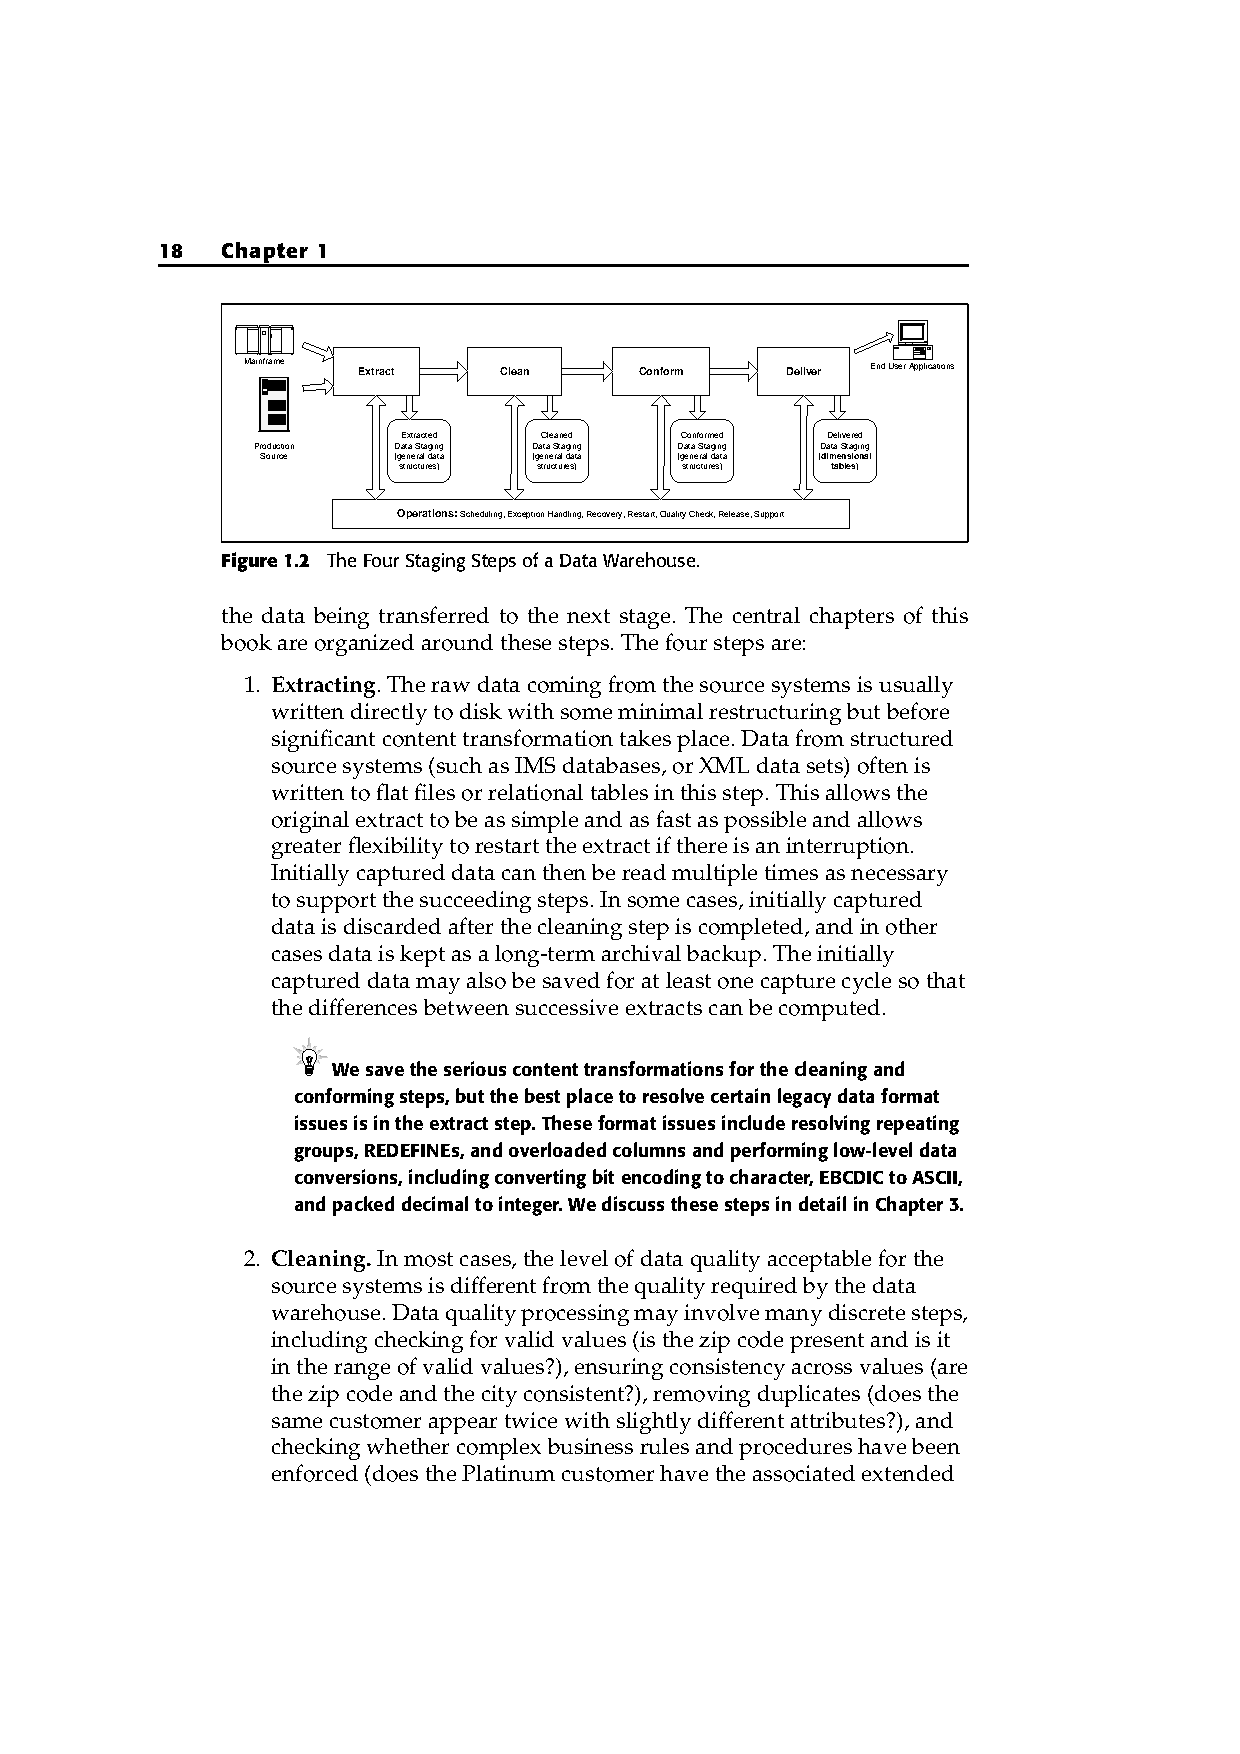
\includegraphics[width=\textwidth, trim={3.5cm 20cm 4.5cm 5cm}, clip]{figures/staging_steps}
\end{frame}

\begin{frame}{The Front Room – Data Access}
    \begin{itemize}
        \item Presentation layer for queries, dashboards, OLAP cubes.
        \item Data marts = measurement-intensive subject areas.
        \item Must be atomic (detail) + aggregated (pyramidal).
        \item Can be centralized or decentralized, but always conformed.
    \end{itemize}
\end{frame}

\section{Mission}
    \begin{frame}{Mission of the Data Warehouse \& ETL Team}
    \textbf{Data Warehouse:}
    \begin{itemize}
        \item Publish data assets to support decision-making.
        \item Deliver reliable, usable, and timely information.
    \end{itemize}
    \textbf{ETL Team:}
    \begin{itemize}
        \item Build the back room.
        \item Add value by cleaning and conforming data.
        \item Protect and document lineage.
        \item Deliver data for querying, reporting, dashboards.
    \end{itemize}
\end{frame}

\begin{frame}{Closing Thoughts}
    \begin{itemize}
        \item Requirements are the foundation of ETL design.
        \item Early architecture decisions shape the entire system.
        \item Back room = preparation; Front room = access.
        \item The ETL team’s mission is strategic to DW success.
    \end{itemize}
\end{frame}

\section{What is PDI?}

\begin{frame}{Pentaho Data Integration in a nutshell}
    \begin{itemize}
    \item \textbf{PDI (a.k.a. Kettle)} = engine + tools for \textbf{Extract, Transform, Load (ETL)}.
    \item Part of the \textbf{Pentaho BI Suite}: analysis (Mondrian), reporting, data mining (Weka), dashboards (CTools), \textit{etc.}
    \item Tight platform services: \textit{authz/authn, scheduling, web services, scalability, failover}.
    \item Community roots \(\rightarrow\) adopted by Pentaho; rapid evolution with frequent releases.
    \end{itemize}
\end{frame}

\begin{frame}{Where PDI fits in the BI stack}
    \begin{columns}[T,onlytextwidth]
        \column{0.55\textwidth}
            \begin{itemize}
                \item \textbf{Data Integration (PDI)} feeds:
                \begin{itemize}
                    \item OLAP (Mondrian)
                    \item Reports (\emph{Pentaho Reporting})
                    \item Data mining (Weka, R/CPython steps)
                    \item Dashboards (CDE/CCC/CDA)
                \end{itemize}
                \item Can run standalone or embedded in the platform.
            \end{itemize}
        \column{0.45\textwidth}
            \begin{block}{Key benefits}
                \begin{itemize}
                    \item Open source ecosystem
                    \item Broad connectivity
                    \item Visual design (Spoon)
                    \item Scales from laptop to cluster
                \end{itemize}
            \end{block}
    \end{columns}
\end{frame}

\begin{frame}{Pentaho Architecture}
    \centering
    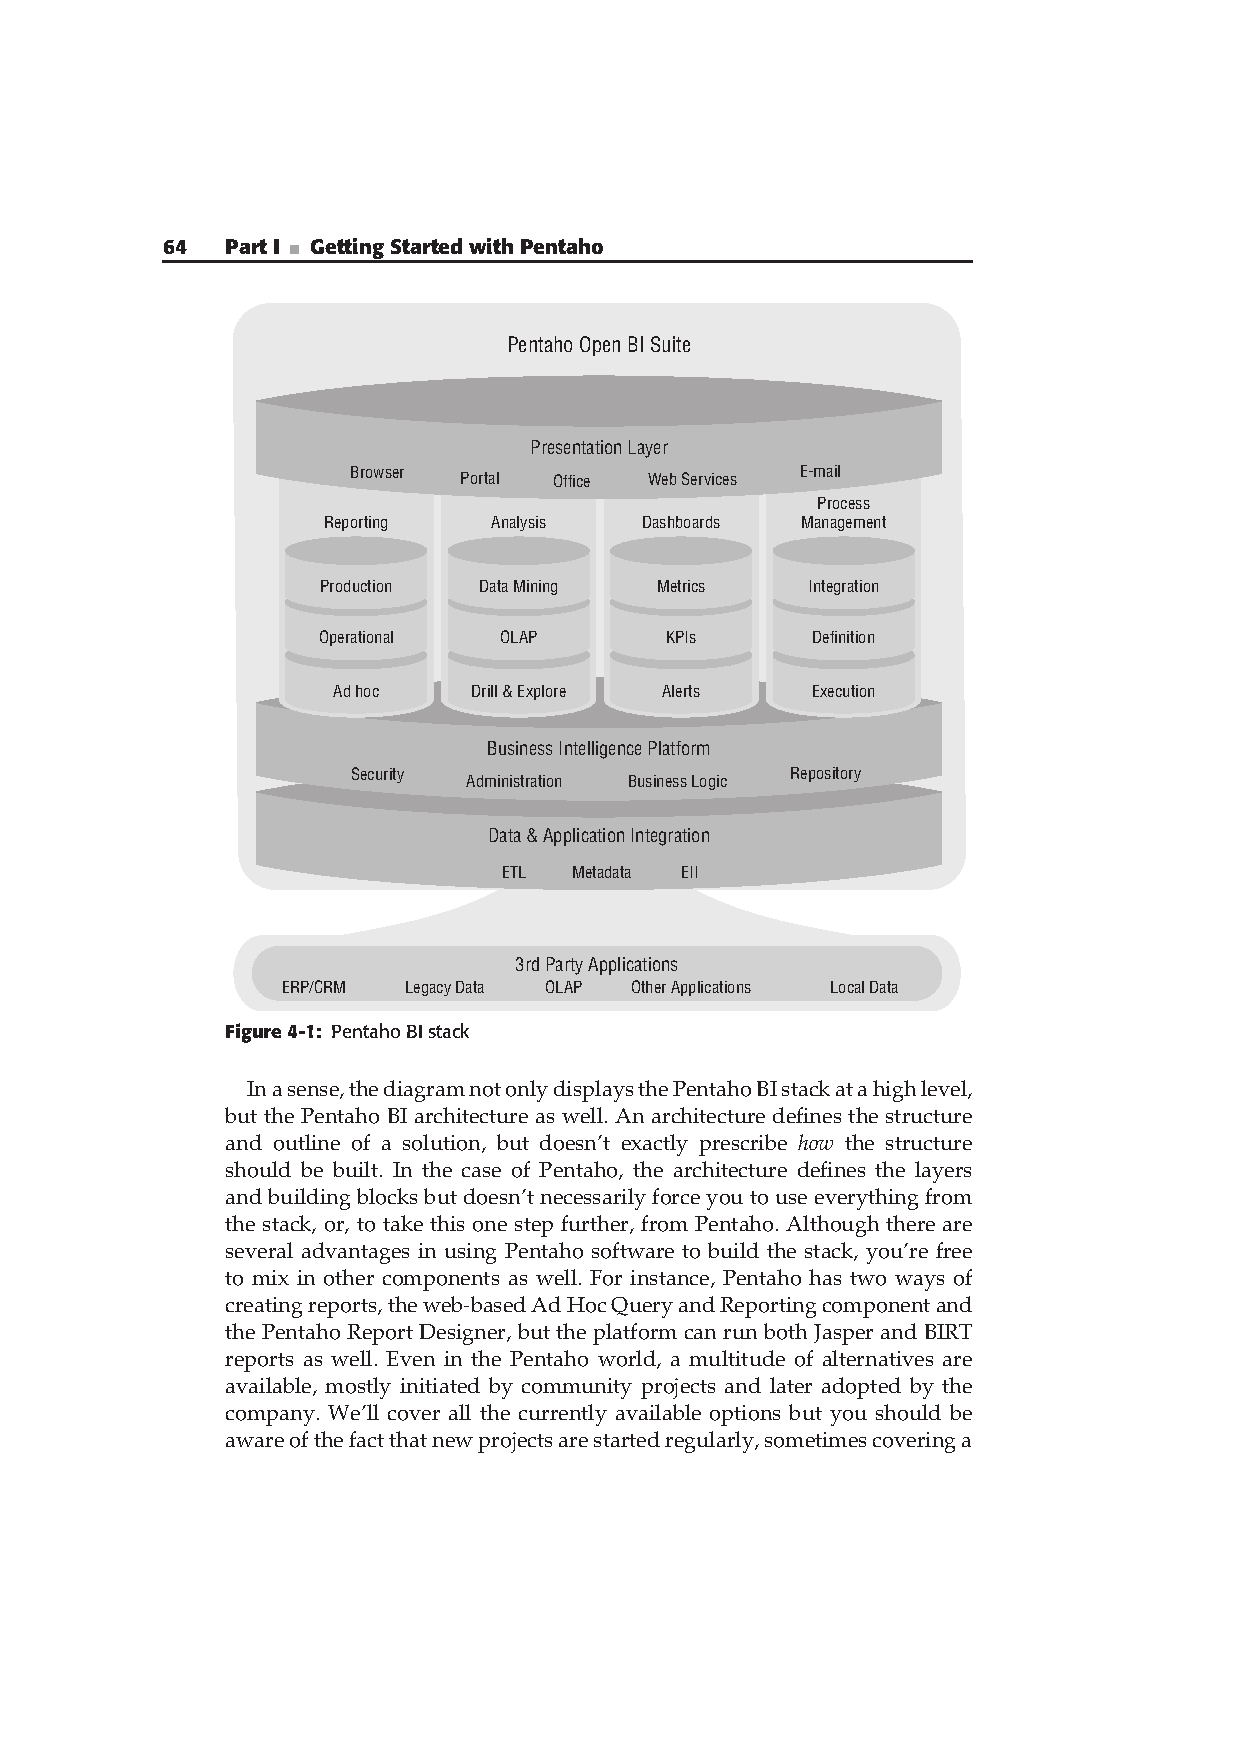
\includegraphics[width=1.1\textheight, trim={3cm 12.5cm 3cm 5cm}, clip]{figures/pentaho_architecture}
\end{frame}

\begin{frame}{Characteristics}
    \begin{itemize}
        \item Data integration: Combining data from different sources to provide a unified view.
        \item Pentaho Data Integration (PDI) offers tools for ETL (Extract, Transform, Load).
        \item Core PDI components: Transformations, Jobs, and the Data Integration Engine.
    \end{itemize}
\end{frame}

\begin{frame}{Data Integration Arquitecture}
    \centering
    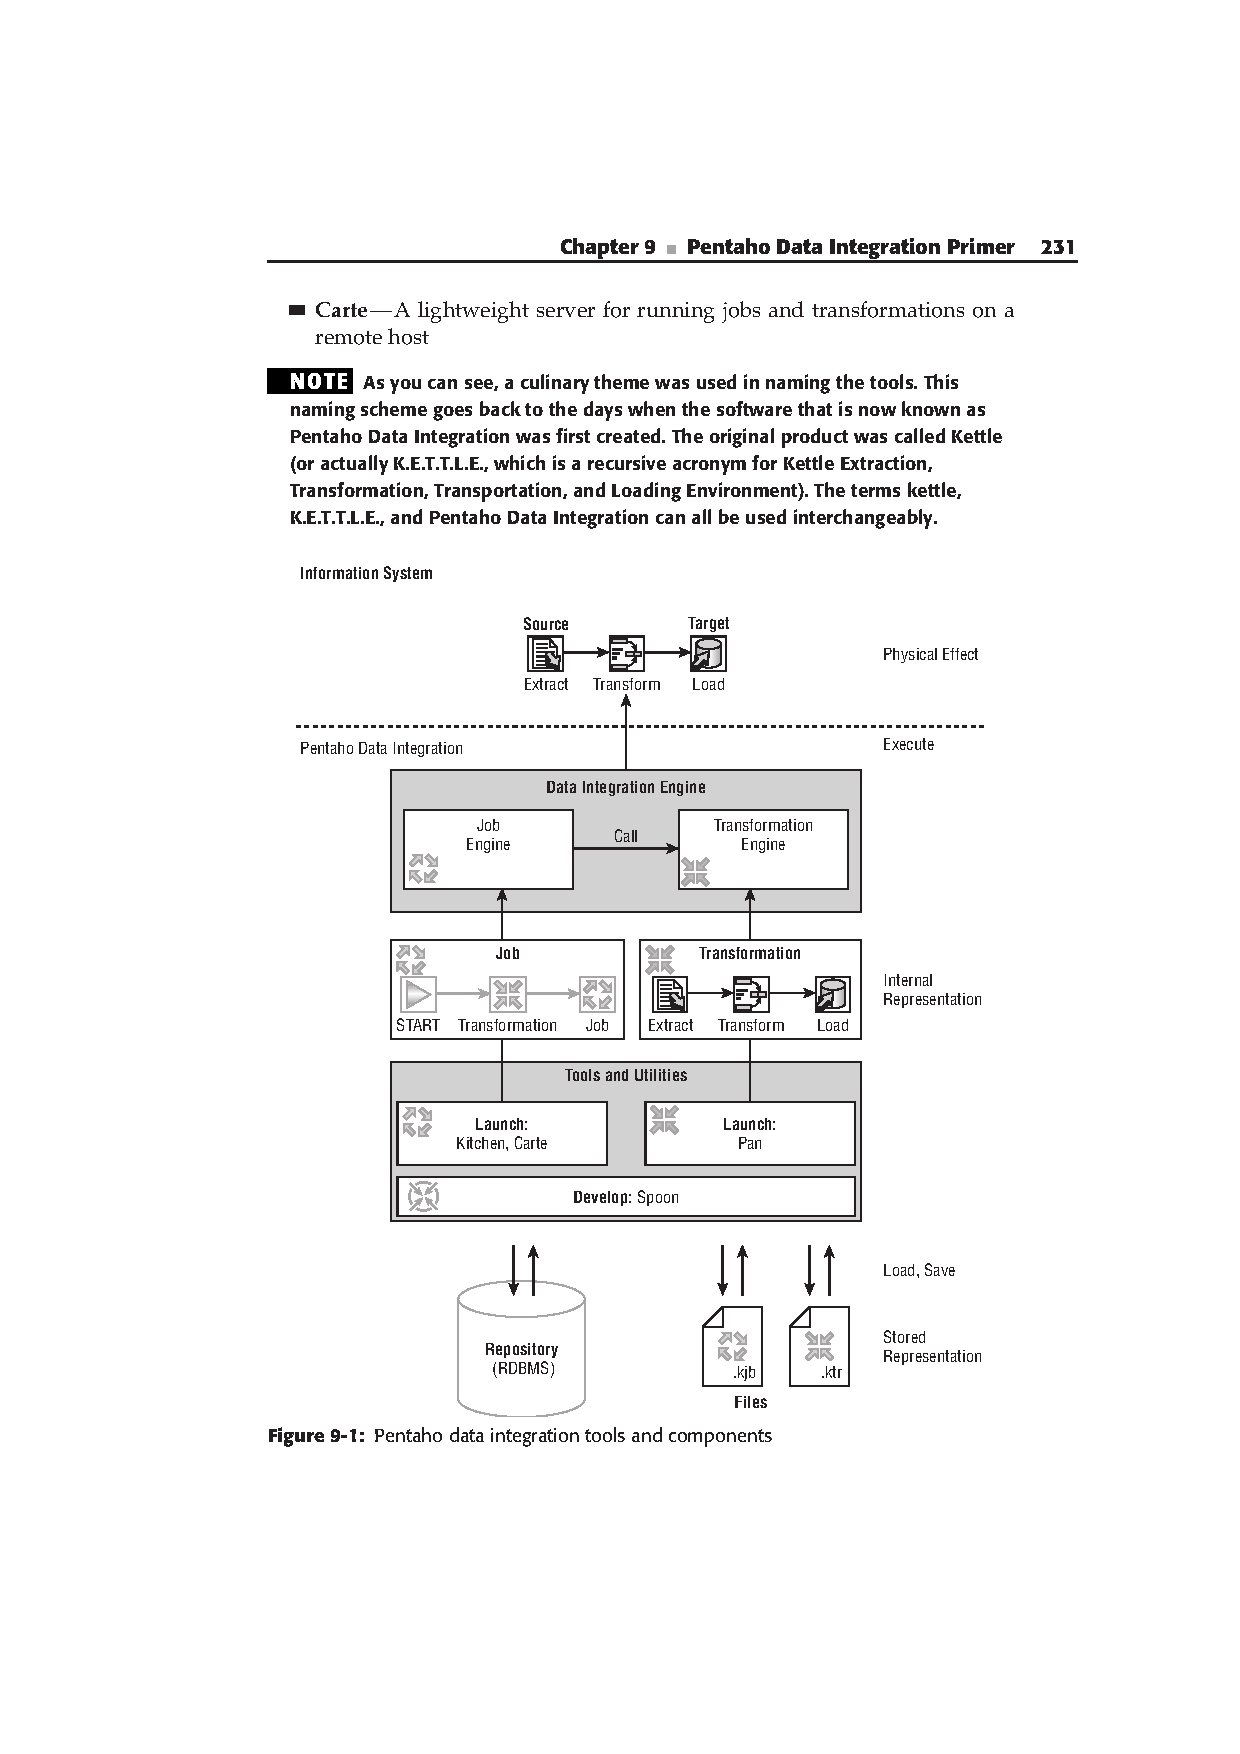
\includegraphics[width=0.95\textheight, trim={3cm 5.55cm 3cm 10cm}, clip]{figures/pdi_architecture}
\end{frame}

\section{What can you do with PDI?}

\begin{frame}{Typical uses (beyond ``just ETL'')}
    \begin{itemize}
        \item \textbf{Load data warehouses/marts} (E\,$\rightarrow$\,T\,$\rightarrow$\,L pipelines, SCD handling).
    \end{itemize}
    \centering
    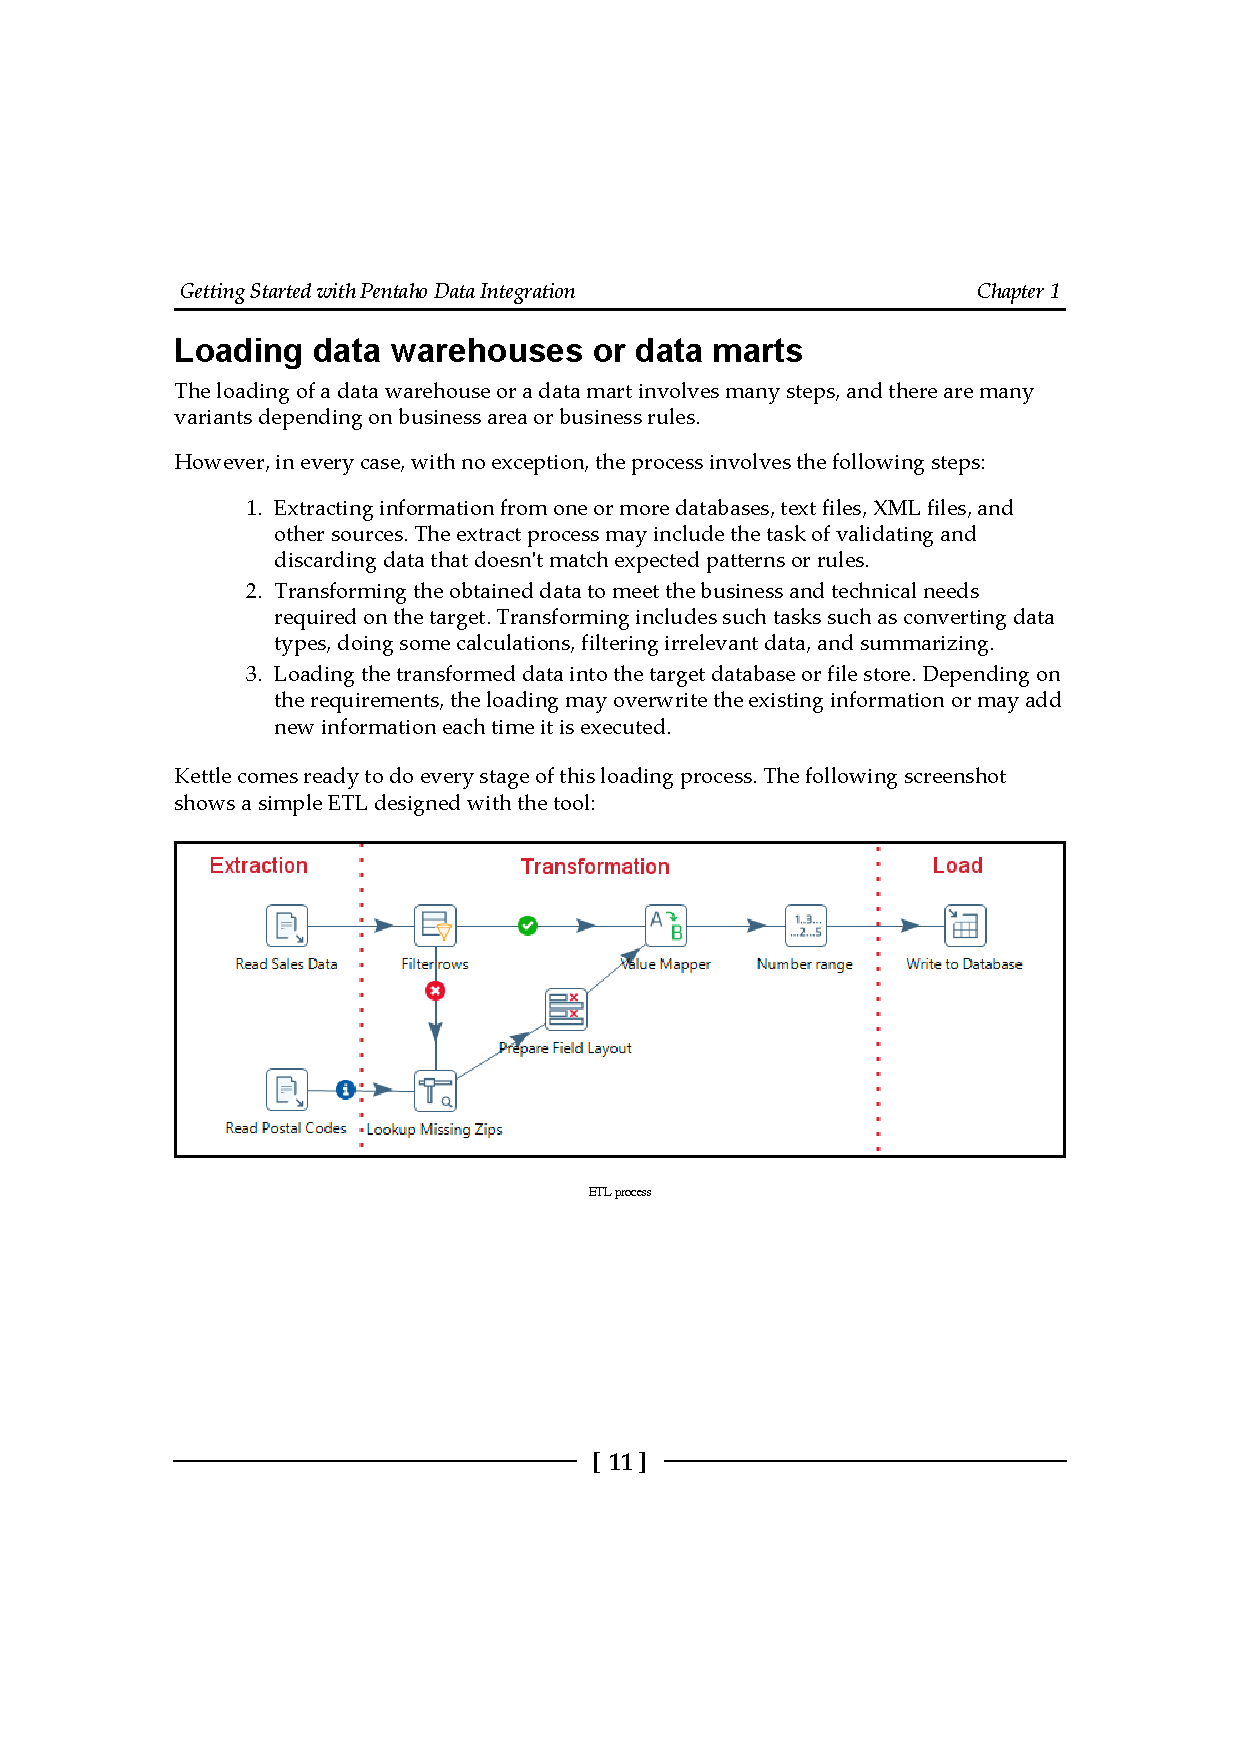
\includegraphics[width=\textwidth, trim={2.5cm 10cm 2.5cm 14cm}, clip]{figures/etl_uses}
\end{frame}

\begin{frame}{Data Integration Activities}
    \begin{itemize}
        \item Extraction: Retrieving data from various sources.
        \item Change Data Capture (CDC): Identifying changes in source data.
        \item Data Staging: Intermediate storage for transformation.
        \item Data Validation and Cleansing: Ensuring data quality.
        \item Key Management and Aggregation.
        \item Dimension and Fact Table Loading.
    \end{itemize}
\end{frame}

\begin{frame}{Typical uses (beyond ``just ETL'')}
    \begin{itemize}
        \item \textbf{Integrate systems} (ERP + CRM, mergers, multi-source unification).
        \item \textbf{Data cleansing} (validation, standardization, deduplication, defaults).
        \item \textbf{Migrations} (schemas/files $\leftrightarrow$ RDBMS/spreadsheets).
        \item \textbf{Exports \& interoperability} (regulatory, inter-dept sharing).
        \item \textbf{Orchestration/automation} (emails, scheduled jobs, preprocess feeds for reports/dashboards).
    \end{itemize}
\end{frame}

\section{Meet Spoon}

\begin{frame}{Pentaho Data Integration Components}
    \begin{itemize}
        \small
        \item \textbf{Kettle}: Data integration engine.
        \item \textbf{Spoon}: Graphical IDE for designing transformations and jobs.
        \item \textbf{Kitchen}: Command-line tool for executing jobs.
        \item \textbf{Pan}: Command-line tool for running transformations.
        \item \textbf{Carte}: Remote execution engine.
    \end{itemize}
    \centering
    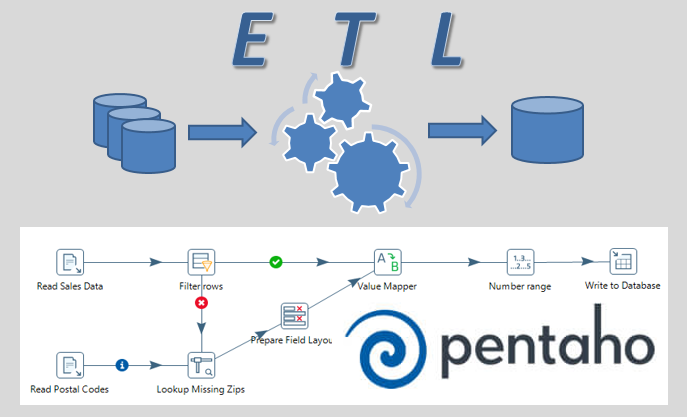
\includegraphics[width=0.6\textwidth]{figures/pdi_components}
\end{frame}

\begin{frame}{Getting Started with Spoon}
    \begin{itemize}
        \small
        \item Launch Spoon and create a new transformation.
        \item Add steps to extract, transform, and load data.
        \item Connect steps using ``hops''.
        \item Preview and execute transformations.
    \end{itemize}
    \vspace{2mm}
    \centering
    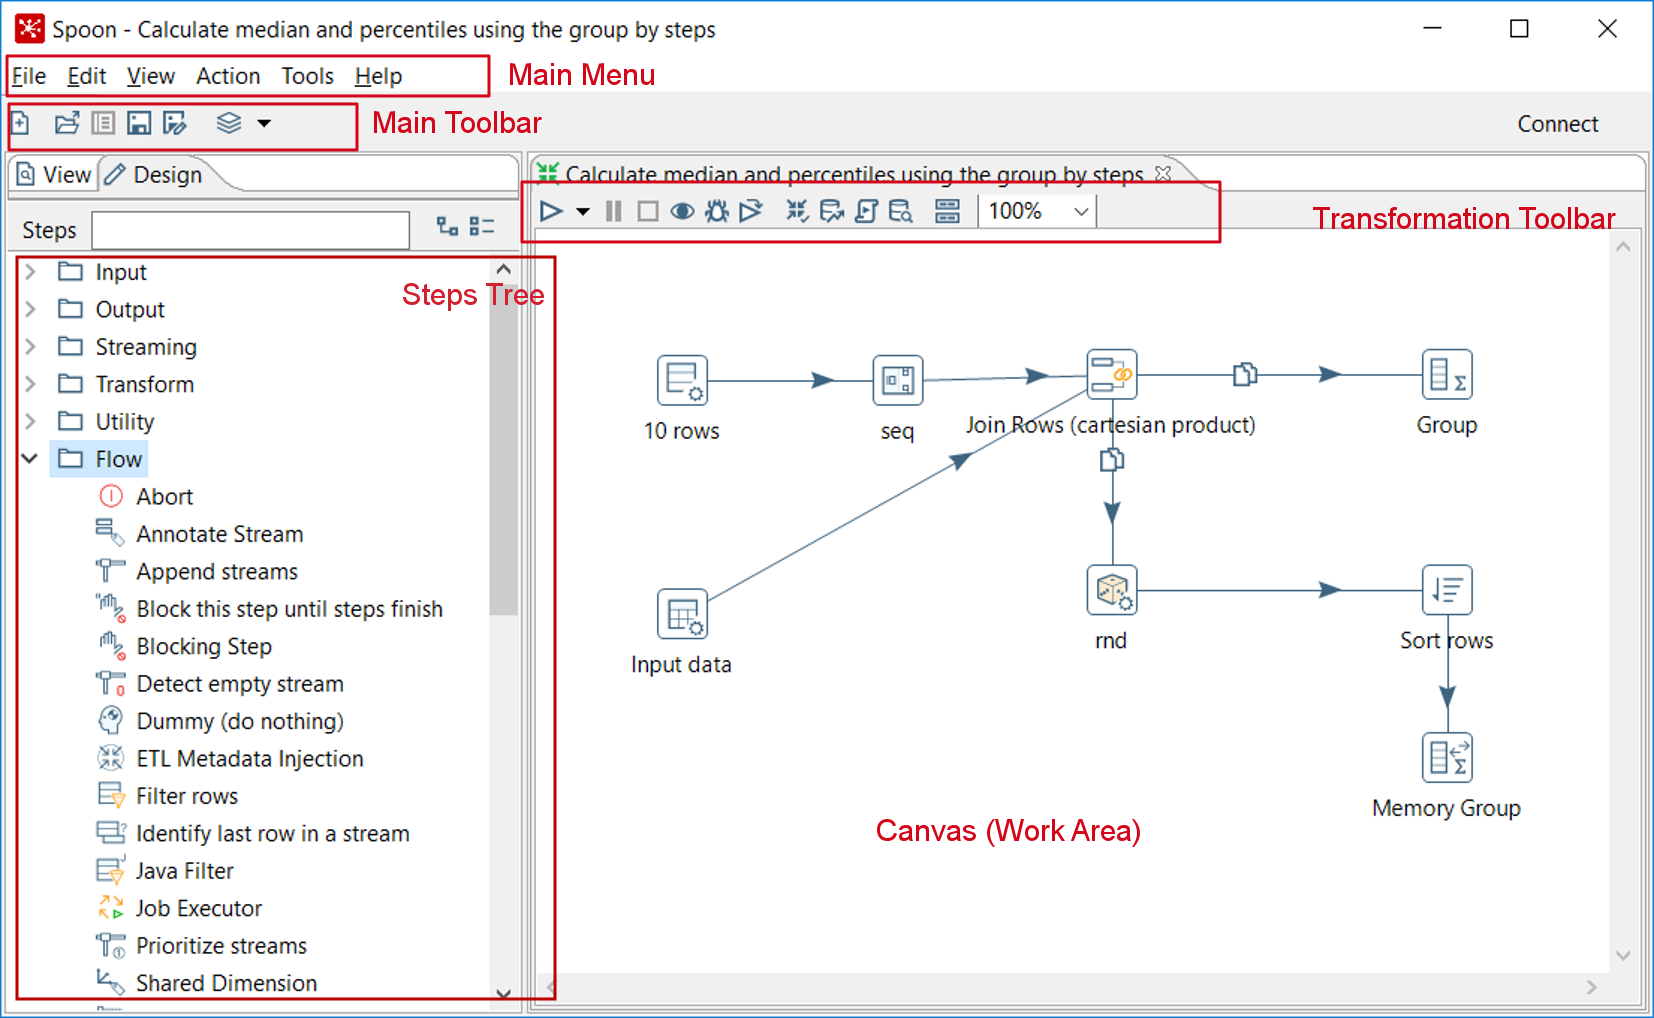
\includegraphics[width=0.6\textwidth]{figures/spoon_ui}
\end{frame}

\begin{frame}{Spoon interface at a glance}
    \begin{columns}[T,onlytextwidth]
    \column{0.55\textwidth}
        \begin{itemize}
            \item \textbf{Main Menu/Toolbar}
            \item \textbf{Design} (Steps tree)
            \item \textbf{View} (structure/logs/metrics)
            \item \textbf{Canvas} (your pipeline graph)
            \item \textbf{Transformation Toolbar} (preview, run, debug)
        \end{itemize}
    \column{0.45\textwidth}
        \begin{block}{Mental model}
            \textbf{Transformation} = \emph{steps} + \emph{hops} (dataflow oriented).\\
            Artifacts are metadata (XML) interpreted by the Kettle engine.
        \end{block}
    \end{columns}
\end{frame}

\begin{frame}{Extending PDI with the Marketplace}
    \begin{itemize}
    \item \textbf{Tools \(\rightarrow\) Marketplace}: browse/install plugins by \emph{Type} and \emph{Maturity}.
    \item Two lanes: \emph{Community} vs \emph{Customer}; stages 1–4 (\emph{lab} \(\rightarrow\) \emph{production-ready}).
    \item Some plugins are EE-only; descriptions indicate availability.
    \end{itemize}
\end{frame}

\section{Your first Transformation}

\begin{frame}{Hello, World! (hands-on in 90 seconds)}
    \begin{enumerate}
        \item \textbf{File \(\rightarrow\) New \(\rightarrow\) Transformation}.
        \item Drag \textbf{Input \(\rightarrow\) Data Grid} to canvas; define a \texttt{name} column and sample rows.
        \item Drag \textbf{Scripting \(\rightarrow\) User Defined Java Expression}; hop from Data Grid to UDJE.
        \item In UDJE, create field
        \texttt{hello\_message = ``Hello, '' + name + ``!''}.
        \item \textbf{Preview} (magnifier icon) on UDJE to sample output; then \textbf{Run}.
    \end{enumerate}
    \begin{block}{Save it}
        \textbf{Edit \(\rightarrow\) Settings} \(\rightarrow\) name, description, extended description \(\rightarrow\) \textbf{File \(\rightarrow\) Save}.
    \end{block}
\end{frame}

\begin{frame}{Summary}
    \begin{itemize}
        \item PDI is a versatile, pluggable \textbf{data integration} engine with a visual designer.
        \item PDI provides tools for efficient ETL processes.
        \item Transformations process data at the record level.
        \item Jobs orchestrate multiple tasks.
        \item Spoon offers a user-friendly interface for development.
        \item You can \textbf{prototype quickly} (preview/run) and scale up as needed.
        \item Marketplace accelerates adoption via \textbf{plugins}—mind the maturity stage.
    \end{itemize}
\end{frame}

%%%%%%%%%%%%%%%%%%%%%%%%%%%%%%%%%%%%%%%%%%%%%%%%%%%%%%%%%%%%%%%%%%%%%%%%%%%%%

\begin{frame}{}
    \centering
    \Huge End of Lecture 5.
\end{frame}

\section*{Takeaways}

% Tim Duncan's Top 5 Fundamental Takeaways of the Today's Class
\begin{frame}{TDT5FTOTC}
    \centering
    
\includegraphics[height=0.9\textheight]{figures/tim.png}
\end{frame}

\begin{frame}{TDT5FTOTC}
    \small
    \begin{enumerate}
        \item[5] PDI, formerly Kettle, is a \textbf{powerful engine and suite of tools} for \textbf{(ETL) processes}, vital for integrating scattered information and a core part of the Pentaho BI Suite. \pause

        \item[4] A \textbf{fundamental architectural decision} in ETL system design is choosing between a \textbf{vendor ETL tool} or \textbf{hand-coding}, significantly impacting development, metadata management, automation, flexibility, and performance. \pause

        \item[3] The \textbf{ETL process}---comprising \textbf{extracting, cleaning, conforming, and delivering} data into a dimensional format---is the core of data warehousing, consuming at least \textbf{70\% of project time, effort, and cost}. \pause

        \item[2] A data warehouse employs a \textbf{two-component architecture}: a \textbf{`back room'} dedicated to data management and preparation, and a \textbf{`front room'} for user data access and analysis. \pause

        \item[1] The \textbf{data warehouse's central mission} is to \textbf{publish organizational data assets for effective decision-making}, with the \textbf{ETL team's core task} being to build the `back room' by cleaning, conforming, documenting lineage, and delivering data dimensionally.
    \end{enumerate}
\end{frame}

\begin{frame}{Database Administration: ETL -- \underline{E}xtraction, \underline{T}ranformation \& \underline{L}oad.}
    \centering
    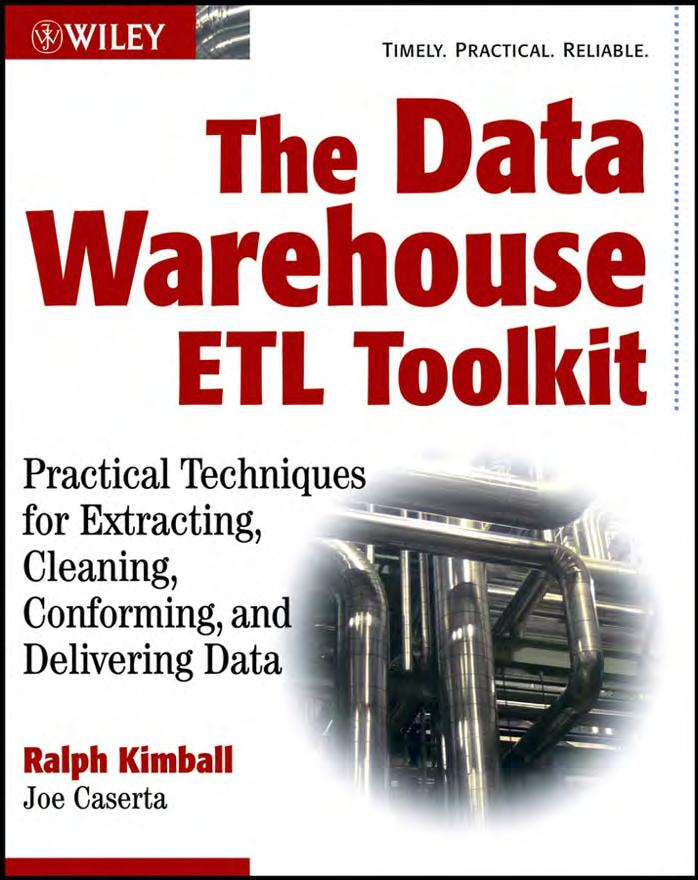
\includegraphics[width=0.3\textwidth]{figures/book_cover5}
    \hspace{5mm}
    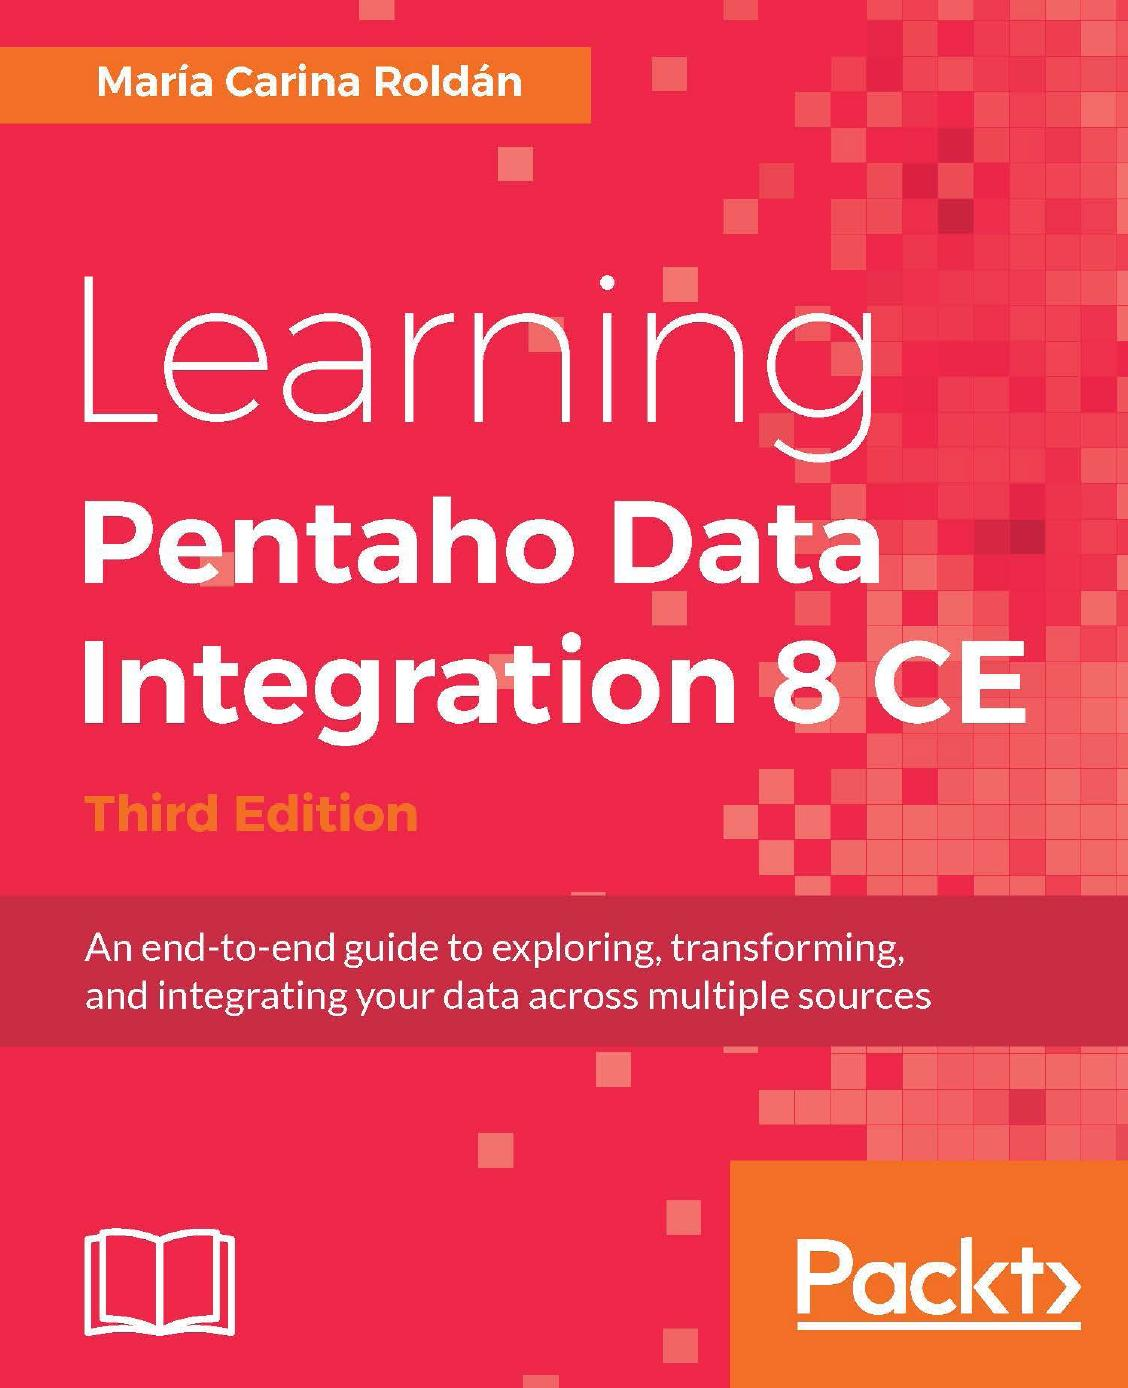
\includegraphics[width=0.3\textwidth]{figures/book_cover6} \\
    \vspace{1mm}
    {
        \scriptsize
        Content has been extracted from \textit{``The Data Warehouse ETL Toolkit''} by Kimball \& Caserta, 2004. Visit \href{https://www.kimballgroup.com/data-warehouse-business-intelligence-resources/books/data-warehouse-dw-etl-toolkit/}{kimballgroup.com}
        and
        \textit{``Learning Pentaho Data Integration 8 CE''} by Roldán, 2018. Visit \href{https://www.oreilly.com/library/view/learning-pentaho-data/9781788292436/a364bedc-72f6-4ccb-94a7-74c499bda3c4.xhtml}{oreilly.com}.
    }
\end{frame}

\end{document}
